\documentclass{beamer}
\usetheme{default}
\beamertemplatenavigationsymbolsempty
\usepackage{rembeamer}
\usepgfplotslibrary{statistics}

\begin{document}

\begin{frame}
  \begin{itemize}
    \item[] 
      Conducting hypothesis testing for differences across more than
      two means and interpreting the results. 
  \end{itemize}
\end{frame}

\begin{frame}
  \frametitle{MLB 2018 Batting Data}
  \centering
  \begin{table}
    \begin{tabular}{@{}llcccc@{}}
      \toprule
      Name & Team & Position & AB & H & OBP  \\
      \cmidrule(r){1-1} \cmidrule(rl){2-4} \cmidrule(rl){3-3}
      \cmidrule(rl){4-4} \cmidrule(rl){5-5} \cmidrule(l){6-6}
      Abreu, J & CWS & IF & 499 & 132 & 0.325 \\
      Acuna Jr., R & ATL & OF & 433 & 127 & 0.366 \\
      Adames, W & TB & IF & 288 & 80 & 0.348 \\
      Adams, M & STL & IF & 306 & 73 & 0.309 \\
      Adduci, J & DET & IF & 176 & 47 & 0.290 \\
      Adrianza, E & MIN & IF & 355 & 84 & 0.301 \\
      \bottomrule 
    \end{tabular}
  \end{table}
\end{frame}

\begin{frame}
  \frametitle{MLB 2018 Batting Data}
  \centering
  \begin{table}
    \begin{tabular}{@{}lccc@{}}
      \toprule
      Position & n & $\mu$ & $\sigma$  \\
      \cmidrule(r){1-1} \cmidrule(rl){2-4} \cmidrule(rl){3-3}
      \cmidrule(rl){4-4} 
      OF & 160 & 0.320 & 0.045 \\
      IF & 205 & 0.318 & 0.038 \\
      C & 64 & 0.302 & 0.038 \\
      \bottomrule 
    \end{tabular}
  \end{table}
\end{frame}

\begin{frame}
  \frametitle{Box Plot - Loans}
  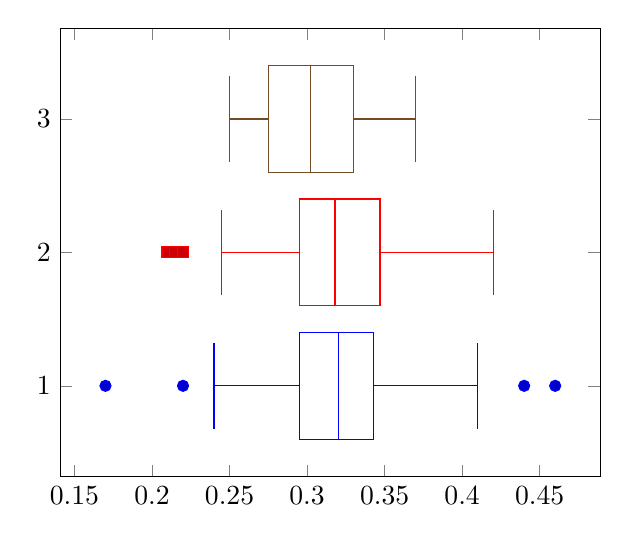
\begin{tikzpicture}
    \begin{axis}
      \addplot+ [
        boxplot prepared={
            lower whisker=0.24,
            lower quartile=0.295,
            median=0.32,
            upper quartile=0.343,
            upper whisker=0.41,
        },
      ] table [row sep=\\,y index=0] {
          data \\ 0.17 \\ 0.22 \\ 0.44 \\ 0.46 \\
      };
      \addplot+ [
        boxplot prepared={
            lower whisker=0.245,
            lower quartile=0.295,
            median=0.318,
            upper quartile=0.347,
            upper whisker=0.42,
        },
      ] table [row sep=\\,y index=0] {
          data \\ 0.21 \\ 0.215 \\ 0.22 \\
      };
      \addplot+ [
        boxplot prepared={
            lower whisker=0.25,
            lower quartile=0.275,
            median=0.302,
            upper quartile=0.33,
            upper whisker=0.37,
        },
      ] table [row sep=\\,y index=0] {
          data \\
      };
    \end{axis}
  \end{tikzpicture}
\end{frame}

\end{document}
